\section{\label{sec:distributedProcessing}Distributed Processing}
The concept of containers introduced so far has been focusing on
self-contained containers. One of the reasons for the {\em container}
concept introduced in Section \ref{sec:containers}, is to provide a
possible split of streaming processes into multiple containers, which
can be deployed in a distributed fashion.

\subsection{Naming Scheme and Services}
Two elements are central for distribution: the concept of remote
services and a naming scheme. Both have essentially been introduced
for local elements in Section \ref{sec:stream-api}.

By extending the naming scheme to incorporate the container
identifiers, we extend this to inter-container communication as shown
in Figure 1.

\begin{figure}
  \begin{center}
    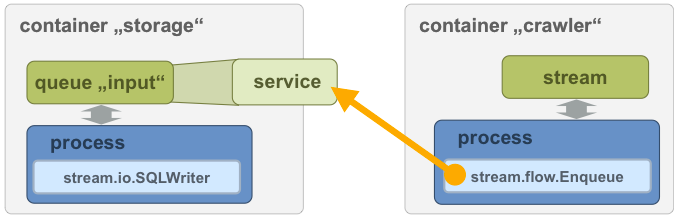
\includegraphics[scale=0.5]{graphics/remote-queue.png}
  \end{center}
  \caption{\label{fig:remote-queue}Inter-Container communcation between {\ttfamily crawler} and {\ttfamily storage.}}
\end{figure}


\subsection{Distributing Containers}
In the simplest case, a container is self-contained and will execute
by itself. However, elements within a container may reference elements
in other containers, allowing for a distributed setup of processes.

A very simple example is given by the two containers in Figure 2. The
container {\ttfamily storage} defines a queue and a process that will
store all elements from that queue in a database.

The second container {\ttfamily crawler} reads data items from Twitter
and sends these to the input queue of the {\ttfamily storage}
container.

\begin{figure}
  \begin{center}
    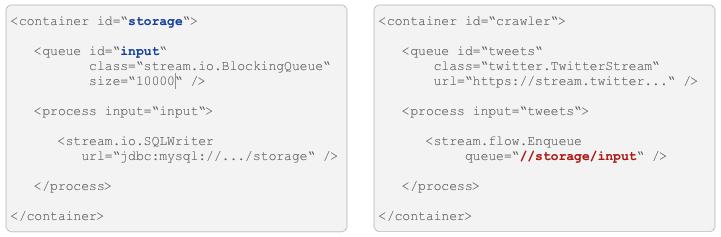
\includegraphics[scale=0.5]{graphics/crawler-storage.png}
  \end{center}
  \caption{\label{fig:crawler-storage} Two simple crawler and storage containers.}
\end{figure}

\subsubsection{Automatic Container Descovery}

By default, each container makes itself available via RMI and responds
to braodcast queries. Therefore no configuration is required as long
as the network infrastructure is capable of distributing the
broadcasts (e.g. in a single ethernet segment).


\subsubsection{Defining Remote Container Connections}

In some situation, the broadcast discover cannot be used or may be
unreliable. To deal with these situations, the naming-service of the
{\em streams} library allows for manually defining references to remote
containers.

The following Figure \ref{fig:container-ref} shows the {\ttfamily
  crawler} container with an explicit RMI reference to the `storage`
container.

\begin{figure}
  \begin{center}
    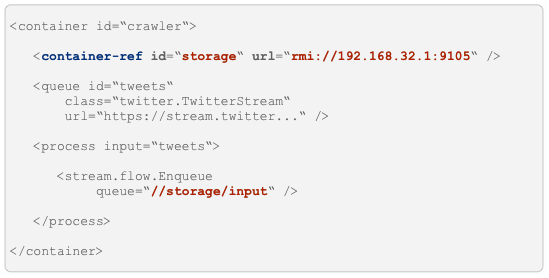
\includegraphics[scale=0.5]{graphics/crawler-explicit-ref.png}
  \end{center}
  \caption{\label{fig:container-ref}Two simple crawler and storage containers.}
\end{figure}
